\documentclass{article}
\pdfpagewidth=8.5in
\pdfpageheight=11in

\usepackage{ijcai26}
\usepackage{times}
% A instalação local do TeX não tem a Courier. Usa a fonte monoespaçada padrão.
\renewcommand{\ttdefault}{cmtt}
\usepackage{url}
\usepackage[hidelinks]{hyperref}
\usepackage[utf8]{inputenc}
\usepackage{graphicx}
\usepackage{amsmath}
\usepackage{booktabs}
\usepackage[brazilian]{babel}

\urlstyle{same}

\renewenvironment{abstract}{\centerline{\Large\bf
Resumo}\vspace{0.5ex}\begin{quote}}{\par\end{quote}\vskip 1ex}

\pdfinfo{
/TemplateVersion (IJCAI.2026.0)
}

\title{Resolvendo o ARC-AGI-1 com LLMs: Fim a Fim e Geração de Código\\(Nível 2)}

\author{
    Lucas Valandro da Rocha
    \affiliations
    Especialização em Inteligência Artificial Avançada, UFRGS
    \emails
    lvalandrorocha@hotmail.com
}

\begin{document}

\maketitle

\begin{abstract}
    O ARC-AGI-1 exige inferir uma regra de transformação de grades a partir de poucos exemplos.
    Este trabalho compara duas formas de usar o Gemini 3.5 Flash Lite, com raciocínio alto, em
    20 tarefas: gerar a grade de saída diretamente (fim a fim) ou gerar um programa Python que
    produz a saída. A geração de código resolveu 17 tarefas, e o fim a fim resolveu 15, com
    custo total de tokens semelhante. Em 16 dessas 17 tarefas, o programa também acertou todos
    os exemplos de treino, e nenhum programa que acertou o treino errou o teste. Isso torna o
    treino um sinal confiável de acerto.
\end{abstract}

\section{Introdução}

O ARC-AGI-1 avalia a capacidade de inferir regras abstratas a partir de poucos
exemplos~\cite{chollet2019arXiv}. Cada tarefa traz alguns pares de grades de entrada e
saída, com cores de 0 a 9, e uma ou mais entradas de teste. A resposta só conta se a grade
inteira estiver correta. As Figuras~\ref{fig:3aa6fb7a} e~\ref{fig:44d8ac46} mostram duas
tarefas do conjunto de treino. Isso é difícil para LLMs por dois motivos. Cada tarefa usa uma regra
nova, que não pode ser memorizada, e o modelo precisa manipular grades célula a célula, uma
operação para a qual a geração de texto token a token não é adequada.

Neste trabalho, usamos o Gemini~\cite{geminiteam2025arXiv} e comparamos duas abordagens descritas
no relatório técnico do ARC Prize~\cite{arcprize2024}. Na abordagem \emph{fim a fim}, o modelo
escreve a grade de resposta. Na \emph{geração de código}, o modelo escreve um programa, e o
computador aplica esse programa à entrada.

\begin{figure}[t]
  \centering
  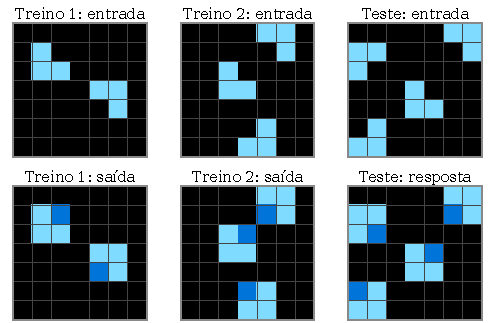
\includegraphics[width=\columnwidth]{figuras/arc_3aa6fb7a.pdf}
  \caption{Tarefa 3aa6fb7a. Cada figura azul-clara em forma de ``L'' ocupa três células de um
  bloco 2$\times$2. A regra é pintar de azul a célula que completa o bloco.}
  \label{fig:3aa6fb7a}
\end{figure}

\begin{figure}[t]
  \centering
  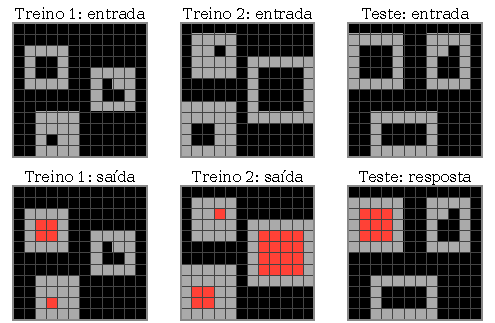
\includegraphics[width=\columnwidth]{figuras/arc_44d8ac46.pdf}
  \caption{Tarefa 44d8ac46. Molduras cinzas cujo buraco interno é quadrado têm o interior
  pintado de vermelho. Buracos que não são quadrados ficam pretos.}
  \label{fig:44d8ac46}
\end{figure}

\section{Método}

O solver foi escrito em Python e lê a lista \texttt{tarefas.txt}. Para cada tarefa, ele envia
ao modelo os pares de treino completos e apenas as entradas de teste, em JSON. As respostas de
teste nunca entram no \emph{prompt}. Os dois \emph{prompts} são os mesmos do notebook do nível~1.

\textbf{Fim a fim.} O \emph{prompt} pede um objeto JSON com uma descrição curta da regra e uma
grade de saída para cada entrada de teste. O solver extrai o JSON da resposta e compara cada
grade com a resposta esperada. Uma resposta fora do formato conta como erro.

\textbf{Geração de código.} O \emph{prompt} pede uma função \texttt{transform(grid)} que use
apenas a biblioteca padrão. O solver extrai o bloco de código e o executa em um processo
separado, com tempo limite de 10~s, primeiro nos exemplos de treino e depois na entrada de
teste. O processo separado impede que um laço infinito ou uma exceção do código gerado
interrompa o experimento. O campo \emph{treino ok} indica que o programa reproduziu todas as
saídas de treino.

\textbf{Medidas.} Para cada tarefa, o solver registra os tokens de entrada, de raciocínio e de
saída, informados pela API, e o tempo da chamada somado ao tempo de execução do código. Cada
resultado é gravado em CSV assim que a tarefa termina, junto com a resposta bruta do modelo.

\section{Experimentos}

Usamos o modelo \texttt{gemini-3.5-flash-lite}, pela API do Google, com nível de raciocínio
alto nas duas abordagens e uma pausa de 1~s entre chamadas. Erros temporários da API, como 429
e 503, seriam repetidos com espera exponencial, mas nenhuma chamada precisou de nova tentativa.
As 20 tarefas são 10 do conjunto de treino e 10 do conjunto de avaliação do ARC-AGI-1. Cada
abordagem fez uma chamada por tarefa, em um total de 40 chamadas. O solver foi construído com o
agente de codificação Claude Code e testado com um modelo falso antes de usar a API.

\begin{table}[h]
  \centering
  \small
  \setlength{\tabcolsep}{2.2pt}
  \begin{tabular}{lrrrrrr}
    \toprule
    Abord. & Resolv. & Treino ok & Entrada & Racioc. & Saída & Tempo (s) \\
    \midrule
    Fim a fim & 15/20 & --    & 53\,706 & 189\,416 & 5\,445 & 538,0 \\
    Código    & 17/20 & 16/20 & 53\,426 & 206\,845 & 8\,516 & 574,2 \\
    \bottomrule
  \end{tabular}
  \caption{Tarefas resolvidas, programas que acertaram todo o treino, total de tokens e tempo
  por abordagem, com raciocínio alto.}
  \label{tab:resultados}
\end{table}

\section{Resultados}

A Tabela~\ref{tab:resultados} mostra que a geração de código resolveu duas tarefas a mais. A
diferença vem do conjunto de treino, em que o código resolveu 10 de 10 e o fim a fim 8 de 10.
No conjunto de avaliação, as duas abordagens resolveram 7 de 10. O custo foi próximo: 248\,567
tokens no fim a fim e 268\,787 no código, ou cerca de 16\,600 e 15\,800 tokens por tarefa
resolvida. Os tokens de raciocínio representam mais de 75\% do total nas duas abordagens.

O treino foi um bom sinal de acerto. As 16 tarefas com \emph{treino ok} foram resolvidas no
teste. Houve também um acerto sem \emph{treino ok}: na tarefa 0a938d79, o programa escolhe a
direção das listras por uma heurística que falha em duas grades de treino, mas que funciona na
entrada de teste.

\textbf{Exemplo de acerto: 44d8ac46.} Nesta tarefa, da Figura~\ref{fig:44d8ac46}, molduras
cinzas fechadas devem ter o interior pintado de vermelho quando o buraco é quadrado. O fim a fim descreveu a regra apenas para buracos de lado
1, 2 ou 4, os tamanhos vistos no treino. Assim, deixou sem pintar um buraco 3$\times$3 do teste e
errou 9 das 144 células, depois de gastar 27\,330 tokens de raciocínio. O programa encontrou os
buracos com uma busca em largura a partir da borda e verificou se cada um é quadrado. Essa regra
vale para qualquer tamanho, e a tarefa foi resolvida com 14\,509 tokens de raciocínio.

\textbf{Exemplo de erro: f5aa3634.} A saída é a figura que aparece repetida na grade, e o seu
tamanho varia entre as tarefas. O programa fixou a altura em 3 linhas e procurou apenas recortes
de largura 3 ou 4. Como a resposta de teste tem 4 linhas, o acerto era impossível, e o programa
também errou os três exemplos de treino. O fim a fim também falhou nessa tarefa. Como o erro no
treino é visível antes da resposta, um laço de correção, como o do nível~3, poderia devolver
essa diferença ao modelo.

\section{Conclusão}

A geração de código com raciocínio alto teve o melhor resultado, com 17 de 20 tarefas, ao custo
de 268\,787 tokens e 574~s, cerca de 8\% a mais de tokens que o fim a fim. A vantagem
apareceu em regras que exigem busca na grade, como na tarefa 44d8ac46, em que o programa
generaliza para tamanhos que não aparecem no treino. O treino também se mostrou um verificador
útil: nenhum programa acertou todo o treino e errou o teste. No nível~1, as mesmas
configurações resolveram 18 tarefas cada uma. Isso indica variação entre execuções, e uma
diferença de duas tarefas deve ser confirmada com repetições. A IA foi usada assim: o Claude
Code ajudou a construir e testar o solver e a redigir este relatório, e os números foram
conferidos com os arquivos em \texttt{resultados/}.

\bibliographystyle{named}
\bibliography{referencias}

\end{document}
